\clearpage
\section{Grundlagen}
\subsection{Grundlagen der Erdvermessung}
Um Karten oder Modelle der Erde zu erstellen, braucht es ein Vermessungssystem welches adäquat die Grösse und Form der Erde widerspiegelt. Wichtig beim Arbeiten mit einem solchen Modell ist, dass man sich bewusst ist, welche Annahmen getroffen wurden und welche Abweichungen aus sowohl der Messmethode als auch dem Modell entstehen. In diesem Kapitel geht es um die Klärung der Grundlagen die zum Verständnis der Funktionsweise des GPS notwendig sind. \cite{geodesy}

\begin{figure}[h]
  \centering
  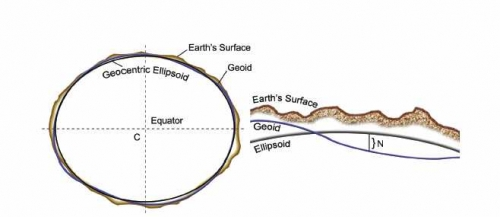
\includegraphics[width=0.8\textwidth]{images/geoid.jpg}
  \caption[Erde, Geoid und Referenzellipsoid]{Verhältnis zwischen der Erdoberfläche, dem Geoiden und einem Referenzellipsoiden. \cite{geodesy}}
  \label{fig:geoid}
\end{figure}

Die Wissenschaft der Erdvermessung - auch Geodäsie - beschäftigt sich mit dem Studium von Grösse und Form der Erde, des Erdgravitationsfeldes und den Veränderungen des eben genannten. Zu den Grundlagen der Geodäsie gehört die Unterscheidung zwischen der physikalischen Erde, dem Geoid und dem Referenzellipsoid. Die physikalische Erde ist die Erde an sich. Der Geoid hat die Form, welche eine von Ozeanen bedeckte Erde, nur unter Einfluss von Gravitation und Rotation annehmen würde. Der Referenzellipsoid ist eine einfache, mathematische Form welche dem Geoid so gut als möglich entspricht. \cite{geodesy}

\subsection{Georeferenzierung}
Die Fähigkeit geografische Positionen genau zu beschreiben ist essentiell für sowohl Karten als auch geografische Informationssysteme. Diesen Prozess nennt man Georeferenzierung.

Eine geografische Position mithilfe von Längen- und Breitengraden auf dem Referenzellipsoiden zu beschreiben ist eine Möglichkeit der Georeferenzierung. Weitere Möglichkeiten wäre zum Beispiel die Verwendung von planaren oder kartesischen Koordinatensystemen. Im Umgang mit GPS werden ausschliesslich Längen- und Breitengrade verwendet, weshalb die weiteren Möglichkeiten im Rahmen dieser Arbeit nicht weiter erläutert werden.

Die Längen- und Breitengrade sind Winkelmessungen wischen dem Zentrum des entsprechenden Ellipsoiden und einem Punkt auf der Oberfläche. Breitengrade (in Englisch latitude) messen dabei den Winkel in Nord-Süd Richtung, Längengrade (in Englisch longitude) den Ost-West Winkel. \cite{georef}

\begin{figure}[h]
  \centering
  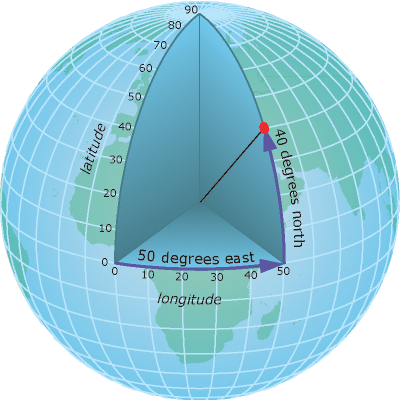
\includegraphics[width=0.5\textwidth]{images/longlat.png}
  \caption[Längen- und Breitengrade]{Lesen von Längen- und Breitengraden \cite{georef}}
  \label{fig:longlat}
\end{figure}

\subsection{World Geodetic System 1984}
Das World Geodetic System 1984 ist das geodätische Referenzsystem welches für GPS Positionsangaben verwendet wird. Als Koordinatenursprung dieses Systems dient das Massenzentrum der Erde. 

Dieses System besteht aus:
\begin{itemize}
	\item einem Referenzellipsoid für Ortsangaben nach geographischer Länge und Breite
	\item einem Geoid
	\item einem Satz dreidimensionaler Koordinaten der zwölf über die Erde verteilten Fundamentalstationen für die Verankerung der zuvor genannten Modelle in der Erdkruste \cite{wsg84}
\end{itemize}

\subsection{Global Positioning System}
GPS Besteht aus drei Segmenten, dem Raumsegment, dem Kontrollsegment und dem Nutzersegment. Das Raumsegment ist so konzipiert, dass es aus 24 bestehen soll, die die Erde in einer Höhe von rund 20200km alle 12 Stunden umrunden. Des weiteren ist das Raumsegment so angelegt, dass immer mindestens 4 Sateliten über einem Mindestelevationswinkel von 15$^\circ$ sichtbar sind. Jeder GPS-Satellit hat mehrere hochgenaue Atomuhren an Bord. Die Uhren arbeiten mit einer Grundfrequenz von 10.23 Mhz, die gebraucht wird, um das von den Satelliten gesendete Signal zu generieren. \cite{leicagps}

\begin{figure}[h]
  \centering
  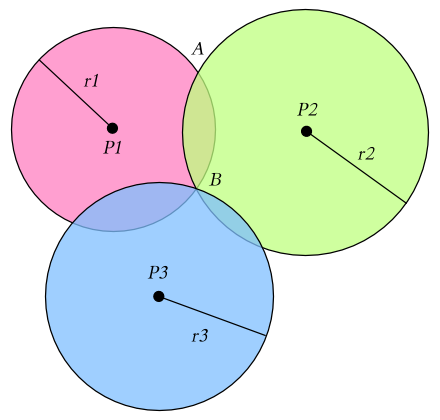
\includegraphics[width=0.6\textwidth]{images/trilateration.png}
  \caption[Trilateration]{Trilateration \cite{trilateration}}
  \label{fig:trilateration}
\end{figure}

Das Kontrollsegment besteht aus einer Hauptkontrollstation, der sogenannten Master Control Station (MCS), 5 Monitorstationen und 4 Telemetriestationen (Bodenantennen) verteilt über 5 Orte, die in etwa auf dem Äquator liegen.\cite{leicagps}

Das Kontrollsegment verfolgt die GPS-Satelliten, aktualisiert ihre Umlaufposition und kalibriert sowie synchronisiert ihre Uhren.\cite{leicagps}

Eine weitere wichtige Funktion ist, die Umlaufbahn eines jeden Satelliten zu bestimmen und seinen Weg für die nächsten 24 Stunden vorherzusagen. Diese Information wird jedem Satelliten eingespeist, um anschliessend von ihm gesendet zu werden. Damit ist der GPS-Empfänger in der Lage zu wissen, wo jeder einzelne Satellit erwartungsgemäss zu finden sein wird.\cite{leicagps}

Das Nutzersegment umfasst all diejenigen, die einen GPS-Empfänger einsetzen, um das GPS-Signal zu empfangen und so ihre Position und / oder Zeit zu bestimmen. Typische Anwendungen innerhalb des Nutzersegments sind die Navigation auf Land für Wanderer, die Bestimmung von Fahrzeugpositionen oder die Vermessung, die Navigation auf See, Navigation in der Luftfahrt, Maschinensteuerung usw. \cite{leicagps}

Die Positionsbestimmung per GPS basiert auf dem Prinzip der Trilateration. Der GPS Empfänger kennt die Position der GPS Sateliten und kann die Distanz zu jedem der Sateliten bestimmen. Wenn die Entfernung zu einem Sateliten bekannt ist, kann die eigene Position nur auf einer Kugelschale mit der Distanz als Radius und dem Sateliten als Mittelpunkt liegen. Durch den Schnitt dreier imaginärer Kugelschalen kann die Empfängerposition bestimmt werden. In der Abbildung \ref{fig:trilateration} ist dieses Prinzip - der einfachheitshalber in 2D - ersichtlich. \cite{leicagps}

\subsection{Distanzberechnung zwischen GPS Koordinaten}
\label{subsec:basicscalcdistance}
Zur Berechnung der Distanz zwischen zwei GPS Koordinaten wurde in dieser Arbeit die Haversine Formel verwendet: \cite{haversine} 

Definitionen:\\
\begin{equation}
\begin{array}{lcl}
\varphi_1, \varphi_2 & = & \text{Breitengrade}\\
\lambda_1, \lambda_2 & = & \text{Längengrade}\\
\Delta\varphi & = & \text{Differenz zwischen den Breitengraden}\\
\Delta\lambda & = & \text{Differenz zwischen den Längengraden}\\
R & = & \text{Radius der Erde}\\
\end{array}
\end{equation}

Berechnung:\\
\begin{equation}
\begin{array}{lcl}
a & = &\sin^2(\frac{\Delta\varphi}{2})+\cos \varphi_1 \cdot \cos \varphi_2 \cdot \sin^2(\frac{\Delta\lambda}{2})\\
c & = & 2 \cdot atan2(\sqrt{a}, \sqrt{(1-a)})\\
d & = & R \cdot c
\end{array}
\end{equation}

Diese Formel verwendet anstelle des Ellipsoiden eine Sphäre was bei grossen Distanzen zu Fehlern führen kann. Bei den Distanzen zwischen Messpunkten von Velotouren oder Wanderungen ist dieser Fehler nicht signifikant. Die Vorteile dieser Formel liegen in der einfachen Implementierbarkeit und der guten Performanz dieser Implementationen. 

\subsection{Das GPX Datenformat}
Das GPX oder GPS Exchange Format ist ein XML Schema zur Darstellung von GPS Daten. Es kann verwendet werden um \flqq Waypoints\frqq, \flqq Tracks\frqq und \flqq Routes\frqq darzustellen. Eine Ansammlung von \flqq Waypoints\frqq kann verwendet werden um eine Menge von Punkten darzustellen die in keinem sequenziellen Zusammenhang zueinander stehen. \flqq Routes\frqq und \flqq Tracks\frqq beinhalten sequenziell angeordnete \flqq Waypoints\frqq. Der Unterschied zwischen den Beiden ist, dass bei einer \flqq route\frqq nur Wegpunkte bei Richtungsänderungen abgebildet sind, den Rest muss sich das System daraus berechnen. Ein \flqq Track\frqq beinhaltet alle aufgezeichneten Punkte. Im Rahmen dieses Projektes werden \flqq Tracks\frqq aufgezeichnet. \cite{gpxwiki} \cite{gpx}

\begin{lstlisting}[language=XML, caption={GPX Beispielfile}]
<?xml version="1.0" ?>
<gpx creator="ch.zhaw.gpstracker" version="1.0" xmlns="http://www.topografix.com/GPX/1/0" xmlns:xsi="http://www.w3.org/2001/XMLSchema-instance" xsi:schemaLocation="http://www.topografix.com/GPX/1/0 http://www.topografix.com/GPX/1/0/gpx.xsd">
    <bounds maxlat="8.28439892" maxlon="8.28439892" minlat="8.28439892" minlon="8.28439892"/>
    <trk>
        <name><![CDATA[Baden-Oberrohrdorf]]></name>
        <trkseg>
            <trkpt lat="47.48865993" lon="8.22070903">
                <ele>379.0</ele>
                <time>2014-06-17T13:38:56Z</time>
                <sym>Dot</sym>
            </trkpt>
            <trkpt lat="47.48859126" lon="8.22059915">
                <ele>378.0</ele>
                <time>2014-06-17T13:39:04Z</time>
                <sym>Dot</sym>
            </trkpt>
            <trkpt lat="47.48381748" lon="8.28364061">
                <ele>410.0</ele>
                <time>2014-06-17T13:57:49Z</time>
                <sym>Dot</sym>
            </trkpt>
        </trkseg>
    </trk>
</gpx>
\end{lstlisting}